\documentclass{article}
\usepackage[french]{babel}
\usepackage[T1]{fontenc}
\usepackage{minted}
\usepackage{graphicx}
\graphicspath{ {./illustrations/} }
\usemintedstyle{gruvbox-light}

\title{TIPE: Apprentissage d'échantillon d'arbres à la gestion d'un village de jeu vidéo}
\author{Eric et Sylvain}
\date{}

\begin{document}
\maketitle
\tableofcontents
\newpage

\section{Carte de jeu}

\subsection{La carte}
La carte de jeu est une matrice carré de chunks. Un chunk est un bloc carré de tuiles, associé à un biome. Une tuile contient un éventuel bâtiment et son élévation.

\begin{listing}[!ht]
\begin{minted}{ocaml}
type tile = Tile of building option * int
type chunk = Chunk of tile array array * biome
type map = chunk array array
\end{minted}
\caption{Typage ocaml de la structure de la carte de jeu}
\end{listing}

\subsection{L'altitude}

L'élevation des tuiles sont calculées à partir d'un bruit de Perlin fractal, c'est à dire constiué d'un empilement de couches successives. Le calcul des produits scalaires nécessaires ainsi que l'empilement des couches est réalisé en parralèle à l'aide de la bibliothèque \mintinline{ocaml}{Domainslib}.

\begin{figure}[h]
  \centering
  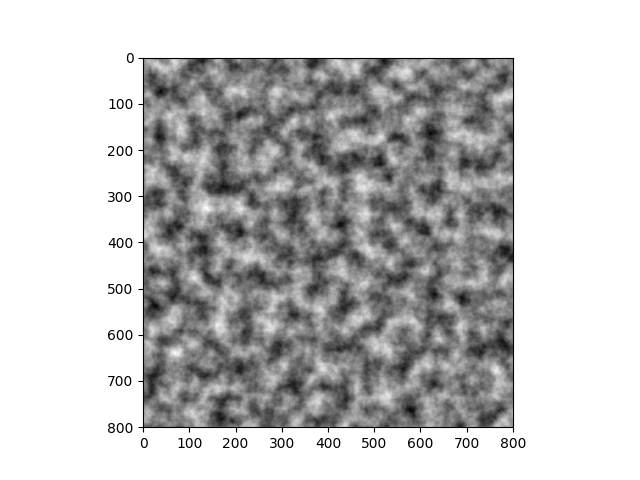
\includegraphics[width=10cm]{perlin_map.png}
  \caption{Un exemple de bruit de Perlin fractal, le foncé représente des valeurs plus élevés}
\end{figure}

Le coût de construction d'un bâtiment dépend notament de l'altitude et du dénivelé moyen du chunk. 

\subsection{Les biomes}

Les biomes disponibles sont le désert, les plaines ou la forêt. Ils ont chacun leurs avantages et leurs inconvénients en terme de coût de construction et de production.

Les biomes sont associés aux chunks, contrairement à l'altitude qui est associée aux tuiles. Les biomes sont générés à l'aide de deux bruits de perlin, un pour l'humidité, un autre pour la végétation. On déduit le biome d'un chunk à l'aide des signes des bruits de Perlin respectifs. On utilise la table de la figure \ref{fig:table_biome} pour en déduire le biome à placer dans le chunk.

\begin{figure}[h]
\begin{center}
\begin{tabular}{c | c  | c}
  & $h < 0$ & $h \ge 0$ \\ 
  \hline
 $v < 0$ & Désert & Plaines \\  
  \hline
 $v \ge 0$ & Plaines & Forêt    
\end{tabular}
\end{center}
\caption{Biome à placer en fonction de l'humidité $h$ et de la végétation $v$}
\label{fig:table_biome}
\end{figure}

Un changement de signe simultané des deux bruits de Perlin autour d'un même point étant rare, des forêts bordant des déserts le sont ainsi tout autant.

\begin{figure}[ht]
  \centering
  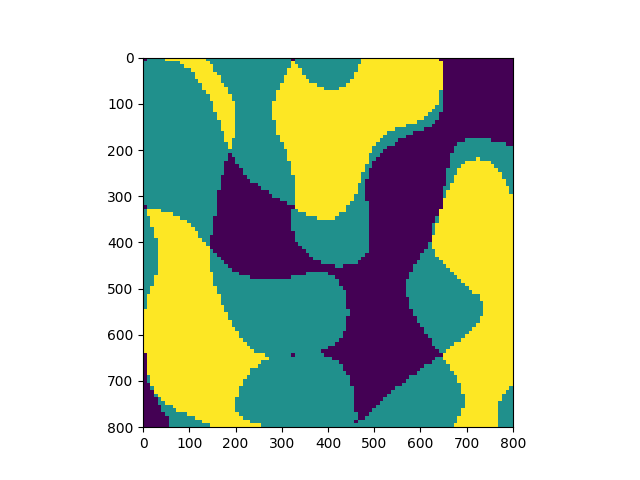
\includegraphics[width=10cm]{biome_map.png}
  \caption{Un exemple de biomes sur une carte, en violet la forêt, en jaune le désert et en vert la plaine.}
\end{figure}

\section{Arbres}

\section{Villages}

\section{Générations}

\end{document}
